\section{Experimental Results}




% problems, with the unicycle dynamics taken from \cite{ReissigWeberRungger_2017_FRR} with nominal disturbance set $\Wnor = [-0.05,0.05]\times [-0.05,0.05]\times [0,0]$. In addition, we assume that the velocity at each dimension of the unicycle will occasionally be perturbed (e.g.\ due to a slippery floor) by disturbances spikes from the set $\Whi=[-d,d]\times [-d,d]\times [0,0]$ for some $d>0.05$. 
%
%\begin{figure}
% 	\centering
%	 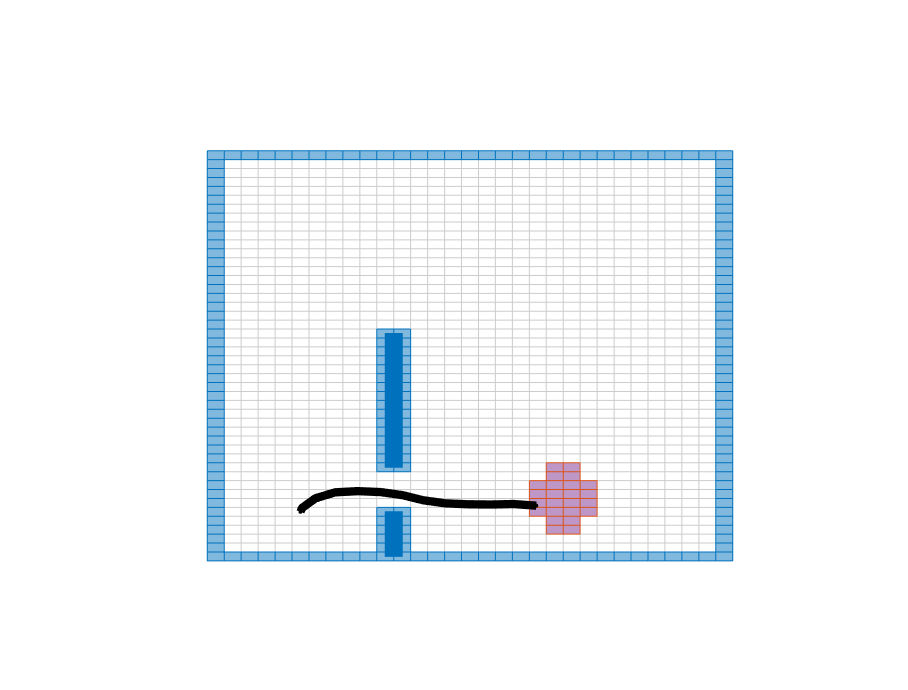
\includegraphics[trim={3.3cm 1.8cm 2.8cm 1.8cm}, clip, width=0.15\textwidth]{figures/naive_controller}
%	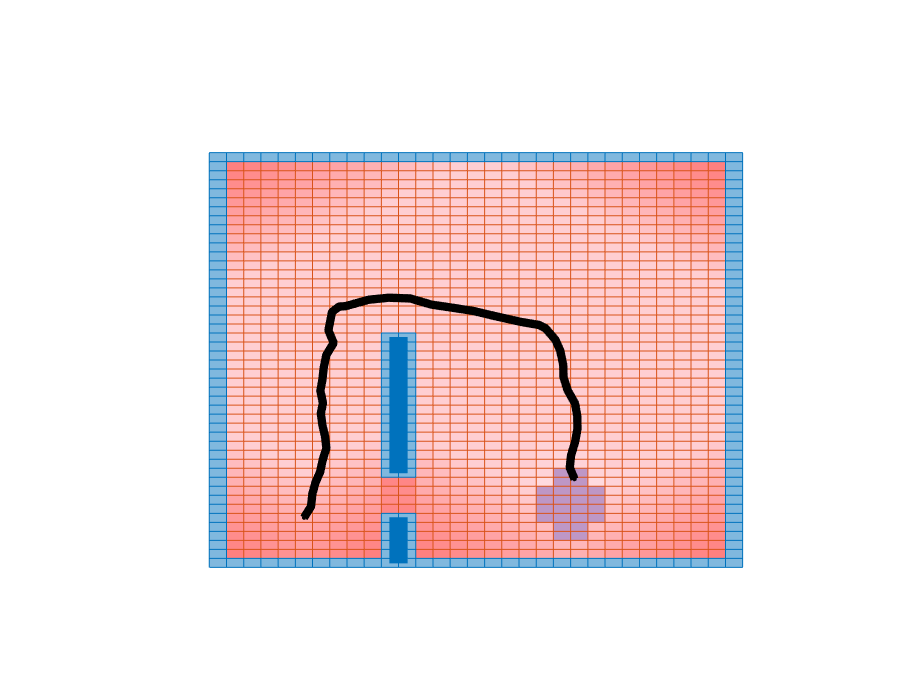
\includegraphics[trim={3.3cm 1.8cm 2.8cm 1.8cm}, clip, width=0.15\textwidth]{figures/ld_005_hd_05_d_70}
% 	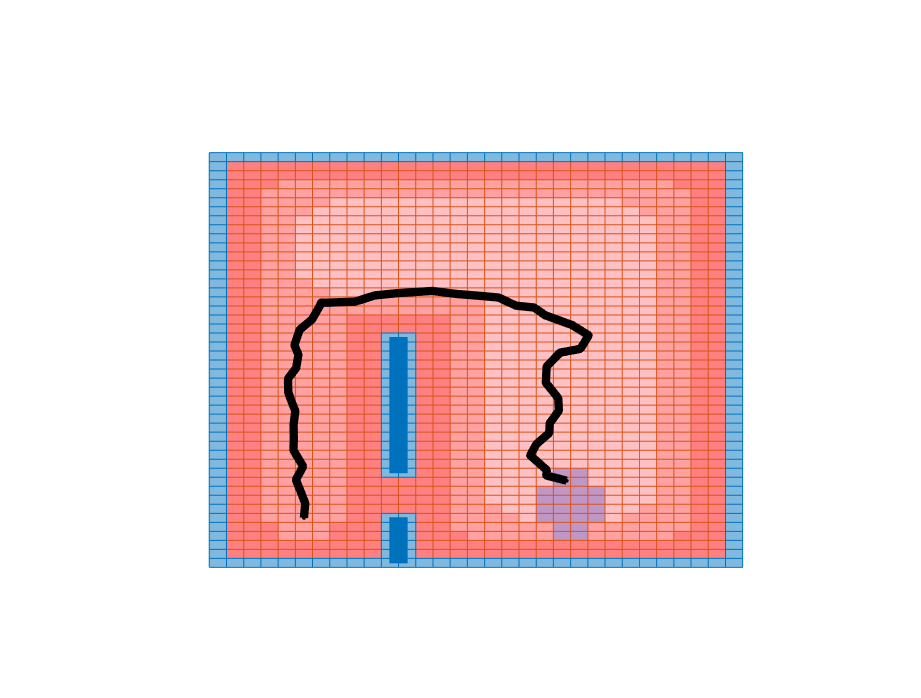
\includegraphics[trim={3.3cm 1.8cm 2.8cm 1.8cm}, clip, width=0.15\textwidth]{figures/ld_0_05_ud_2_d_70_r_3}
% 	\vspace{-0.3cm}
%	 \caption{\textbf{Reach-while-avoid control}: Classical ABCD using SCOTS (left);
%	 Resilient ABCD with $d=0.5$ (middle) and $d=2$ (right). Lower resilient states are indicated in darker shade than higher resilient states. Strategies through the wide passage are more resilient.
%	 }
%	 \label{fig:plots}
%\end{figure}
%
%\smallskip
%\noindent\textbf{Reach-While-Avoid.}
%We first consider a simple \emph{reach-while-avoid} specification for the unicycle robot as depicted in Fig.~\ref{fig:plots}.
%In this example, the robot must pass through either a narrow or a wide passage to avoid the obstacles (blue) and reach the target (purple).
%We have implemented this synthesis problem as a Parity specification with three colors -- color $2$ assigned to target states and color $1$ assigned to all other states, while color $0$ is kept empty.
%To enforce obstacle avoidance, we manipulate the computed abstract transition system to self-loop in obstacle states on all normal and disturbance edges. Hence, whenever the robot visits an obstacle state \emph{once}, it is forced to stay there forever and thereby visits color $1$ infinitely often which violates the specification. Fig.~\ref{fig:plots} depicts the path of the robot to the target; the computed controller additionally ensures that the target is (re-) visited infinitely often, by looping inside it.
%
%Under normal disturbances, both passages are equally safe. Therefore, the original SCOTS algorithm returns a strategy which guides the robot along the shortest path to the target, passing the small passage (Fig.~\ref{fig:plots} (left)).
%% 
%In contrast, RESCOTS synthesizes a controller which enforces the shortest path through the less risky wider passage (Fig.~\ref{fig:plots} (middle and right)) while assuming occasional disturbance spikes with $d=0.5$ (middle) and $d=2$ (right), respectively. 
%It can be observed that the smaller $\Whi$ the higher the number of resilience values: 16 for $d=0.5$ (middle) as opposed to 3 for $d=2$ (right).
%I.e., the larger the set $\Whi$, the lower the number of high disturbance spikes which pushes the robot from a state in the middle of the work space into an obstacle.
%
%
%\begin{figure}
%
%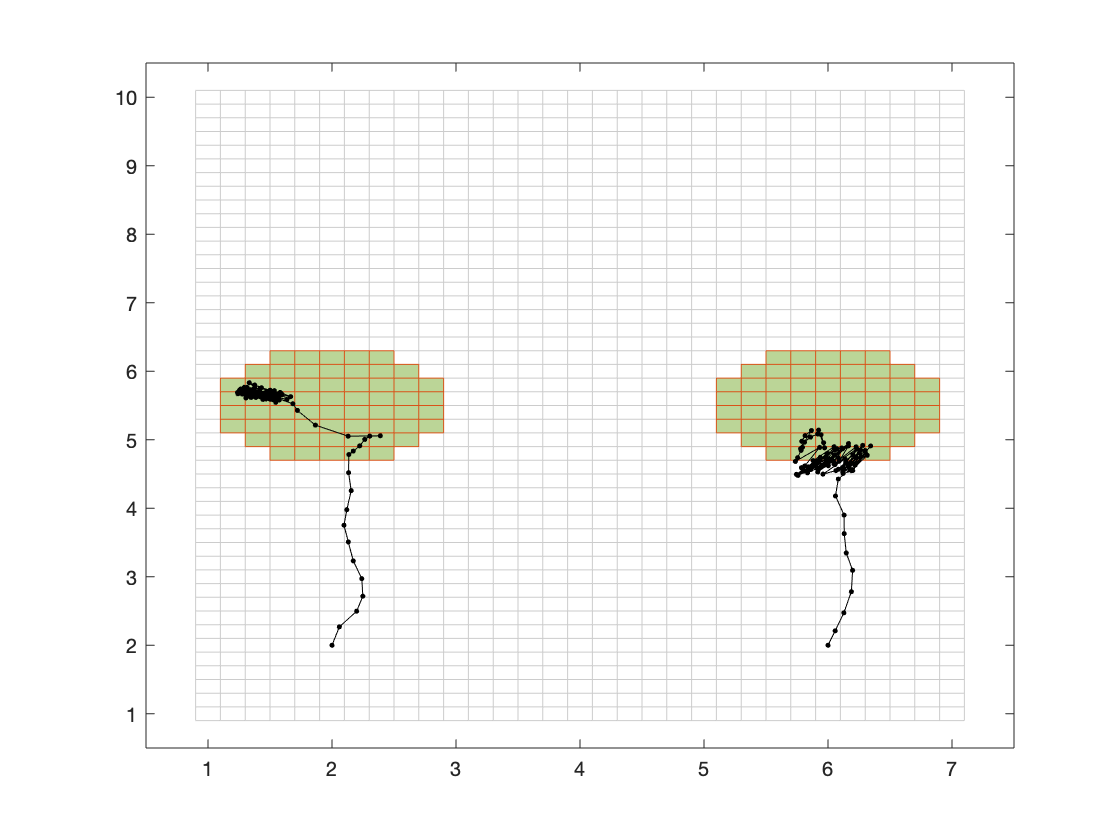
\includegraphics[trim={5.5cm 3.4cm 4.8cm 2.5cm}, clip, width=0.23\textwidth]{figures/newexample_left}
%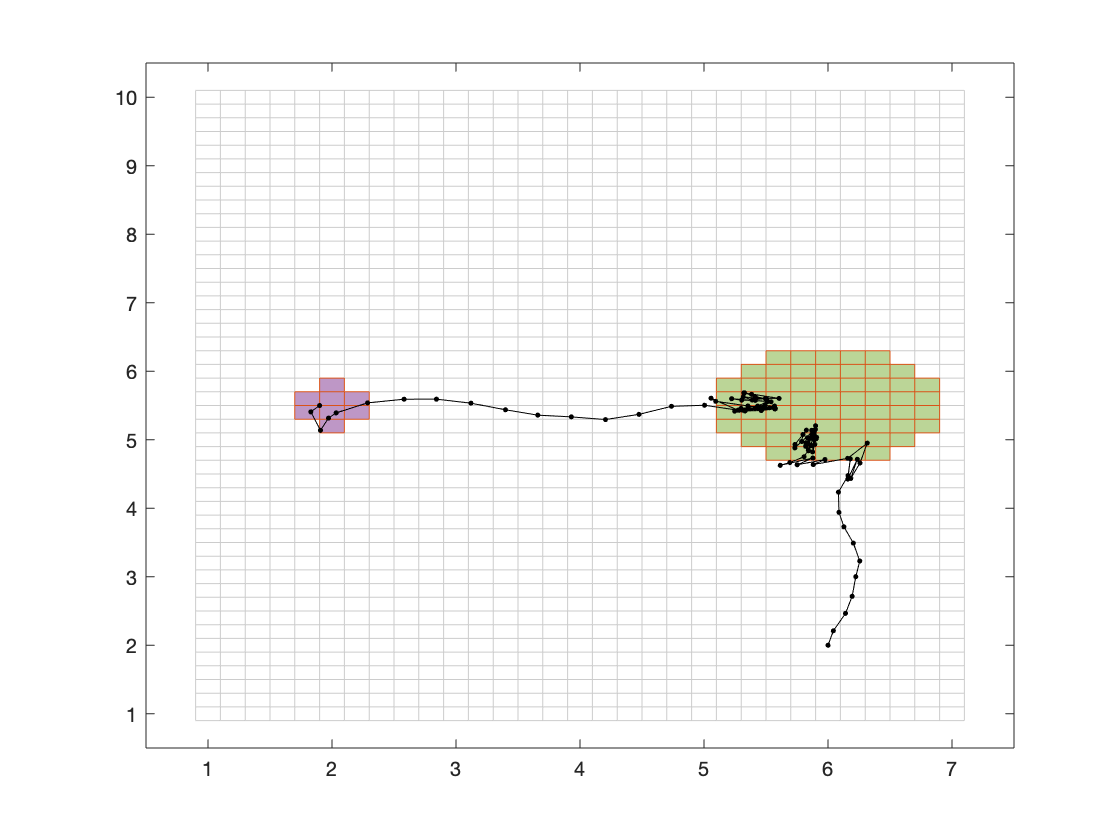
\includegraphics[trim={5.5cm 3.4cm 4.8cm 2.5cm}, clip, width=0.23\textwidth]{figures/newexample_right}
%\vspace{-0.3cm}
%\caption{\textbf{Co-Büchi vs. Büchi objectives}: 
%	 Fulfilling a Co-Büchi objective for the left and a Büchi objective for the right target. $\omega$ and $\omega+1$ resilient states are indicated in white and green, respectively. %For $d=2$ the Büchi objective is more resilient.
%	 }\label{fig:plots_ex2}
%	 \vspace{-0.3cm}
%\end{figure}
%
%\smallskip
%\noindent\textbf{Eventuality properties.}
%To illustrate the control strategies computed by RESCOT in the presence of eventuality properties we consider a $3$-color parity specification for the unicycle robot in a bounded open space with no obstacles.
%Here, color $0$ is assigned to the left target ($T_l$), color $2$ is assigned to the right target ($T_r$) and color $1$ is assigned to every other state. 
%
%This specification imposes two possible strategies for the robot: (i)  move to $T_l$ (color 0) and stay inside $T_l$ forever, or (ii) visit at least one state in $T_r$ infinitely often. Hence, the robot can choose between a Co-Büchi specification w.r.t.\ $T_l$ and a Büchi specification w.r.t.\ $T_r$.
%
%The difference of enforced trajectories depending on the Co-Büchi and the Büchi specification is depicted in Fig.~\ref{fig:plots_ex2} (left). We see that the robot does not make an effort to get to the interior of $T_r$, as being pushed out by a disturbance infinitely often (and then moving back in) does not violate the specification. However, the robot makes an effort to stay inside $T_l$; leaving $T_l$ infinitely often would violate the specification. 
%
%For the scenario depicted in Fig.~\ref{fig:plots_ex2} (left) both specifications are satisfyable with resilience $\omega+1$ and the robot chooses the target closest to its starting point. If we decrease the size of the left target (Fig.~\ref{fig:plots_ex2} (right)), only the Büchi specification for $T_r$ is satisfyable with resilience $\omega+1$ and is therefore chosen by the robot from any initial state.
%% Formally, we therefore get resilience  $\omega+1$ states in the interior of $T_r$ and $T_l$ for small disturbance spikes $d=0.1$ (Fig.~\ref{fig:plots_ex2} (left)), while we only get resilience $\omega$ in all $T_l$ states for larger disturbance spikes $d=0.2$ (Fig.~\ref{fig:plots_ex2} (right)).
%% In this case we therefore see that the robot always moves to $T_r$ even when starting close to $T_l$ to optimize its resilience.
%
%
%\begin{figure}
% 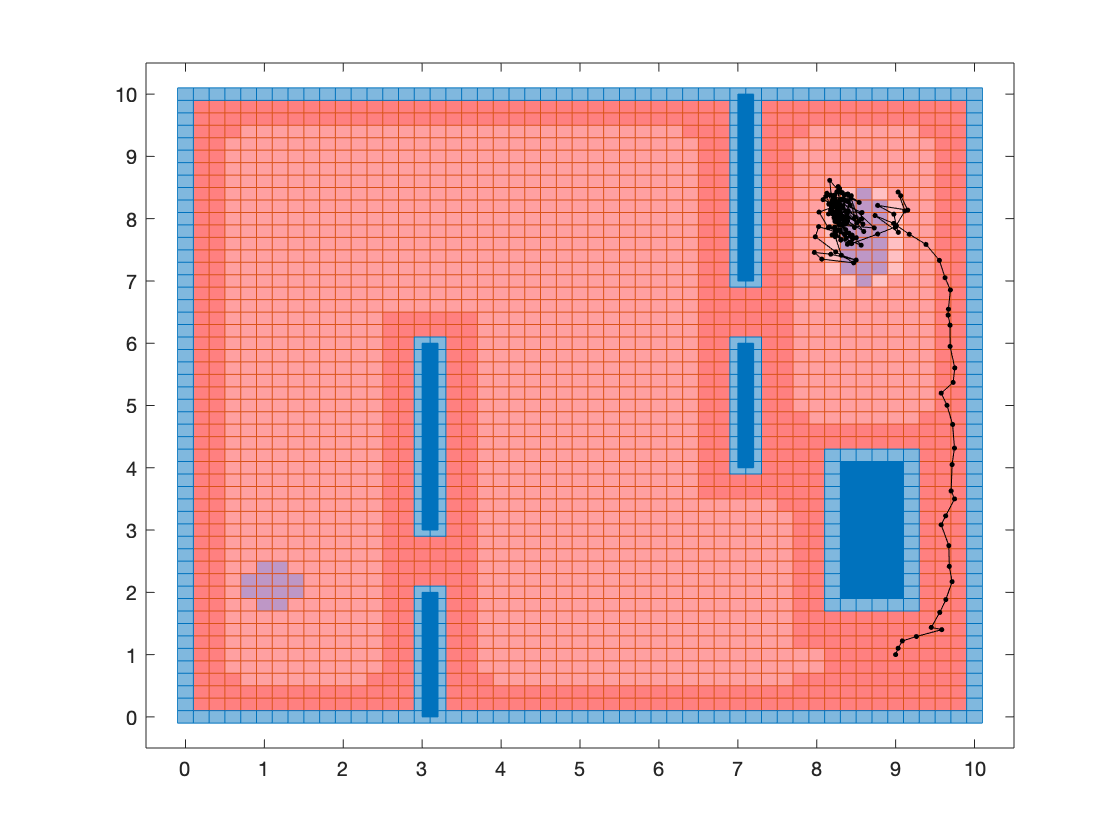
\includegraphics[trim={5.8cm 3.5cm 4.8cm 2.5cm}, clip, width=0.23\textwidth]{figures/Rabin_right_high}\hfill
%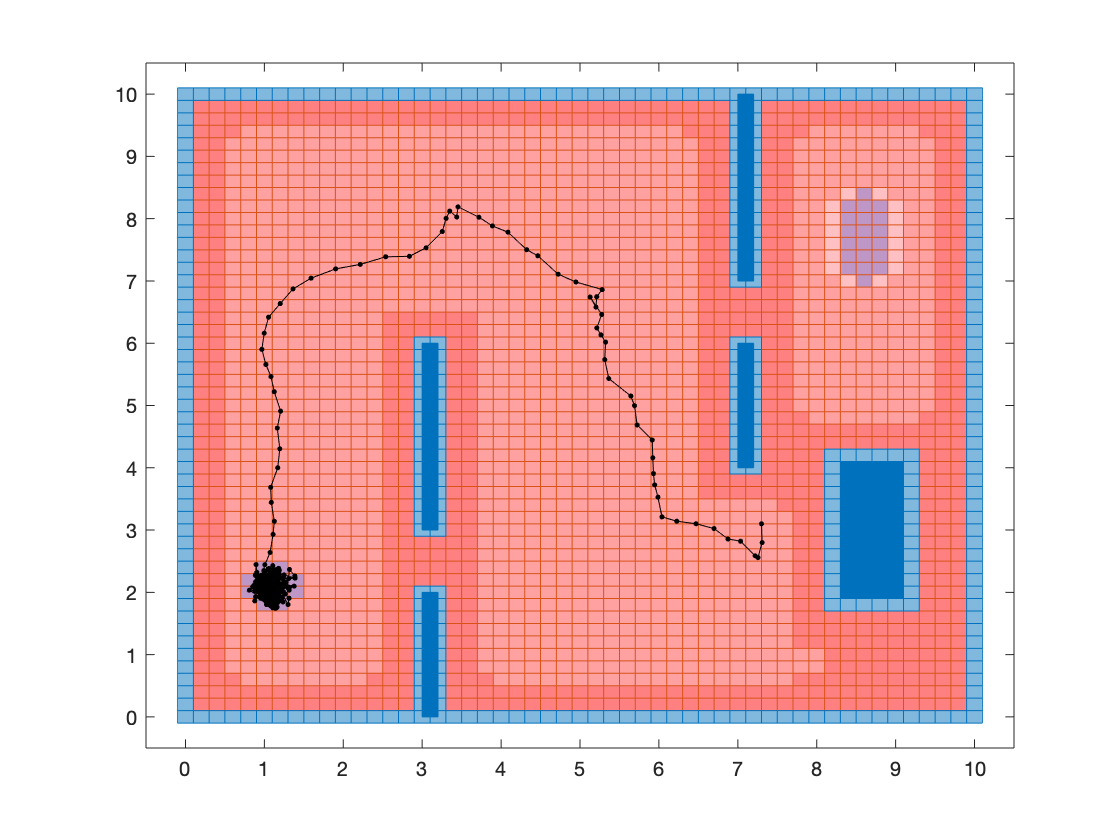
\includegraphics[trim={5.8cm 3.5cm 4.8cm 2.5cm}, clip, width=0.23\textwidth]{figures/Rabin_init2_left_low}
%\vspace{-0.3cm}
%	 \caption{Synthesis problem of Fig.~\ref{fig:plots_ex2} under additional obstacle avoidance. All states (including target states) have finite resilience. Here targets are entirely chosen based on the reaching path resilience.
%	 }
%	 \label{fig:plots_ex3}
%\end{figure}
%
%\smallskip
%\noindent\textbf{Eventuality properties and finite resilience.}
%As a last experiment, we add obstacles to the scenario in Fig.~\ref{fig:plots_ex2} as shown in Fig.~\ref{fig:plots_ex3}. This results in a $4$-color parity game where, as before, color $0$ is assigned to the left target ($T_l$), color $2$ is assigned to the right target ($T_r$) and color $1$ is assigned to every other state. Now we additional assign color $3$ to all obstacles (blue) and again enforce obstacle avoidance by self-loops within those states.
%
%In this case we see that all states, including the states inside the targets, get a finite resilience. This is due to the fact that a finite number of successive disturbances can force the robot to bump into the wall. Choosing to satisfy the Büchi objective (i.e., move to $T_r$) is therefore not more resilient then choosing to satisfy the Co-Büchi objective. In particular, 
%the controller avoids passing the risky, dark red passage for moving to $T_r$ and chooses to go to $T_l$ instead, which is further away (see Fig.~\ref{fig:plots_ex3} (right)). However, if it is already inside the risky dark red region, it prefers to move to $T_r$, which is closer.
%
%
